% --------------------------------------------------------------------------- %
%               _ _       _ _        _                       _                %
%            __| (_) __ _(_) |_ __ _| |  _ __ ___  _   _ ___(_) ___           %
%           / _` | |/ _` | | __/ _` | | | '_ ` _ \| | | / __| |/ __|          %
%          | (_| | | (_| | | || (_| | | | | | | | | |_| \__ \ | (__           %
%           \__,_|_|\__, |_|\__\__,_|_| |_| |_| |_|\__,_|___/_|\___|          %
%                   |___/                                                     %
%                                                                             %
%           _           _                                   _                 %
%          (_)_ __  ___| |_ _ __ _   _ _ __ ___   ___ _ __ | |_ ___           %
%          | | '_ \/ __| __| '__| | | | '_ ` _ \ / _ \ '_ \| __/ __|          %
%          | | | | \__ \ |_| |  | |_| | | | | | |  __/ | | | |_\__ \          %
%          |_|_| |_|___/\__|_|   \__,_|_| |_| |_|\___|_| |_|\__|___/          %
% --------------------------------------------------------------------------- %
\chapter{Aesthetic Experience, Complex Music Systems, and the Metaverse}
\label{sec: theory}
%\markboth{}{Aesthetic Experience, Complex Music Systems, and the Metaverse}
\epigraph{\emph{In actual experience, there is never any such isolated singular object or event; an object or event is always a special part, phase, or aspect, of an environing experienced world—a situation'}}{\citep[p. 67]{dewey1934}}

\begin{figure}
    \centering
    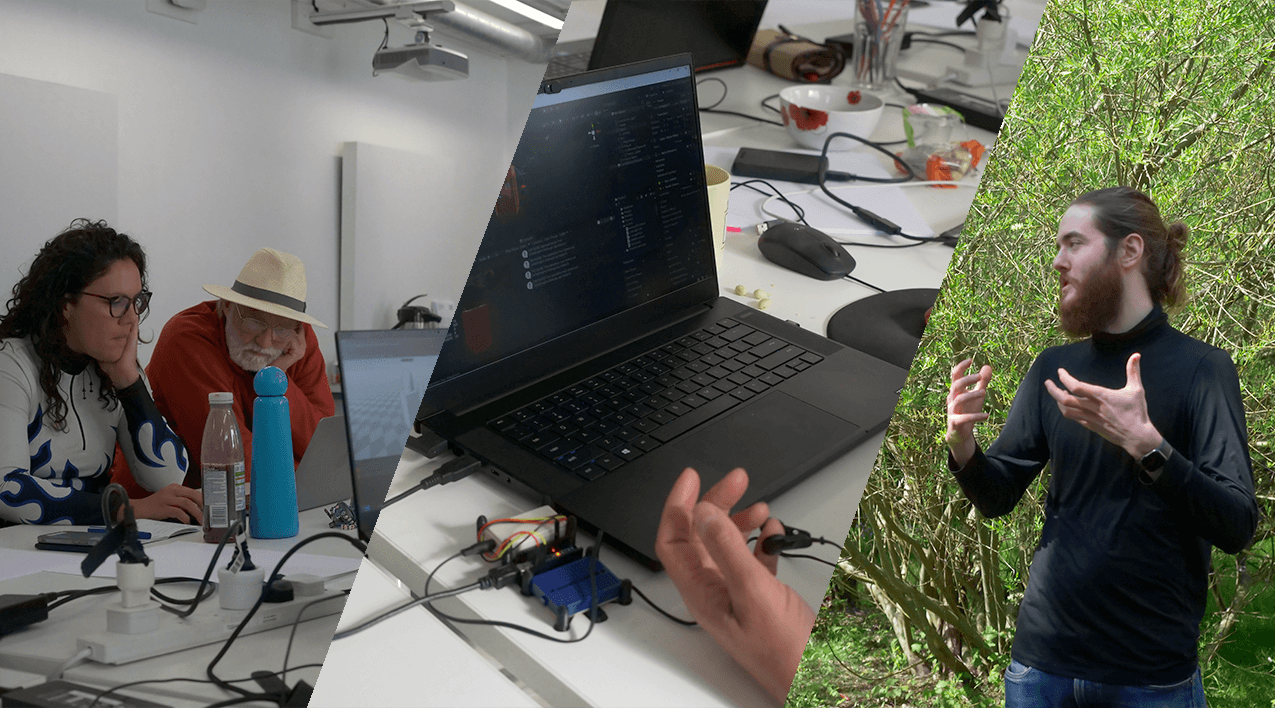
\includegraphics[width=1\linewidth]{03-theory/chapter-fig.png}
    \captionsetup{labelformat=empty}
    \caption[\autoref*{sec: theory}'s page-figure: Three photographs from the Sensory Cartographies project, (from \citefullauthor{tonn2017}, \citeyear{tonn2017})]{}
\end{figure}

\clearpage
% --------------------------------------------------------------------------- %
\section{Summary}\label{sec: theory-summary}
In the previous chapter, I outlined the problematic origins of \gls{ar} technology from within the U.S. military-industrial complex. This origination from within neo-colonial and capitalist modes of thought has had a compounded effect on the form that \gls{ar} takes today: predominantly it is sought as a `visual overlay' device. Despite this, clearly limiting perspective, we are seeing increased use of \gls{ar} as a medium for the creation of meaningful experiences through interactive artwork. Though fairly established in modes of visual art because of this predominant form, its use in sound related art forms has been limited. As a result, the present thesis promotes a sensory-process agnostic \footnote{That is to say, not limited to visual sensory displays, and not limited to augmentation processes} conceptualisation of \gls{ar}, by using the more holistic definition `real-time computationally mediated perception' \citep{kiefer2018} moving forwards. 

But first, we must carve out a space for the consideration of \gls{ar} as a medium for new forms of aesthetic experience in specifically sound-driven art forms, such as composition, performance, installation, and instrument building. This chapter does so by first outlining what we mean by aesthetic experience. In delving deeper into contemporary theories of mind and embodiment, I propose (as others have done), that an enactivist approach to design guided by the 4E's (embodied, embedded, enactive, extended) may be beneficial when considering the material, embodied, and spatial nature of interactive music systems, and more specifically, those that employ \gls{ar}. From this foothold, the chapter goes on to considers a trio of theoretical lenses through which to consider the process of mediation in \gls{ar} experience, and the types of aesthetic experience this results in. Namely, by exploring the concept of complexity in the \textbf{materiality} of interactive musical systems; enactivist approaches to considering \textbf{embodiment} in XR systems; and a brief discussion on why the Metaverse in its current form is not the ideal \textbf{space} for artistic expression.



% --------------------------------------------------------------------------- %
\section{Knowledge and Aesthetic Experience}\label{sec: theory-experience}
What is experience when it comes to art; how does it relate to epistemological practice? To address this question, the present thesis draws from the work of the American pragmatist John Dewey (1859-1952). In his 1934 text, Art as Experience, Dewey argues that the production and consumption of art faces a crisis. After having been historically coupled in an constitutive relationship with the processes of everyday sociocultural life, it is being increasingly separated from these `conditions of origin and operation in experience' \citep{dewey1934}, in a way that places art upon a remote pedestal. Dewey describes this as a product of the growth of capitalism. On proposing what they term Dewey Aesthetics, Leddy and Puolakka write:
\begin{quote}
    `Nothing about machine production per se makes worker satisfaction impossible. It is private control of forces of production for private gain that impoverishes our lives. When art is merely the `beauty parlor of civilization,' both art and civilization are insecure. We can only organize the proletariat into the social system via a revolution that affects the imagination and emotions of [hu]man[kind]. Art is not secure until the proletariat are free in their productive activity and until they can enjoy the fruits of their labor. To do this, the material of art should be drawn from all sources, and art should be accessible to all.' \citeyearpar{leddy2021}
\end{quote}
From this standpoint, art can serve as an emancipatory force for positive social change; but only on the condition that it is first brought back to the `origin and operation' of everyday experience — through the democratisation of a wider corpus of artistic media, tools, and social contexts in which these are deployed. In the 21st century, we could mistake this for already having happened. The increasing availability of ubiquitous technologies such as the internet, wearables, smartphones, powerful computers and software have shifted artistic production closer to the site of everyday sociocultural life — from the studio to the bedroom. Yet in doing so, has art really been knocked from its pedestal and been re-integrated into, and resituated to arise from everyday life? 

Today, the fabric through which art tends to be disseminated and therefore consumed, social media, arguably operates within this same capitalist framework, the vocabulary having shifted from art in the museum, to content on our feeds. Despite making art more accessible to produce and consume, the capitalist logic of surplus extraction the centre of the algorithms that determine our interaction with social media vies to keeps art separate from everyday life. Central to this is that instead of being centralised in a museum or gallery, it is the concept of the pedestal itself that we should venerate. We must each curate our own museums and galleries, our own feeds.

\begin{figure}[ht]
    \centering
    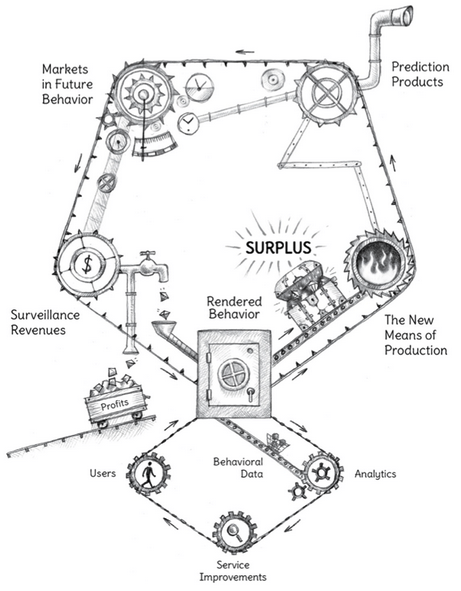
\includegraphics[width=.75\linewidth]{03-theory/zuboff2019.png}
    \captionsetup{justification=centering,margin=1.5cm}
    \caption{The Discovery of Behavioural Surplus \citep[in][]{zuboff2019}}\label{fig: zuboff2019}
\end{figure}

The unavoidable truth of these platforms however, is that they are not solely focused on fostering individual or even collective curation of democratised art/content. They still employ the capitalist framework at their core. This extractivist profit motive defines the algorithmic fabric of online `content creation' (production), and resultant social media `engagement` (consumption) through mass data harvesting and advertisement selling. The longer users are engaged on a platform (Facebook, Instagram, Twitter, YouTube, TikTok), the more likely they are to generate profits for the platform via advert click/tap-throughs. Our feeds are interspersed with adverts and sponsored posts that have been carefully curated to maximise the potential click/tap-through rate of their victims. Soshana Zuboff defines this as arising from a `market of human behavioural futures' \citeyearpar{zuboff2019} in her book Surveillance Capitalism. Through this surveillance, large amounts of behavioural, affective, and personal data (termed behavioural surplus by Zuboff) are `skimmed' off the top of our engagement with these platforms, and sold to agencies that match this personal data with products/content you are most likely to engage with. How could it be argued that that the production and consumption of art / content on such platforms is not governed by `private gain' at our expense? 

\begin{figure}[ht]
    \centering
    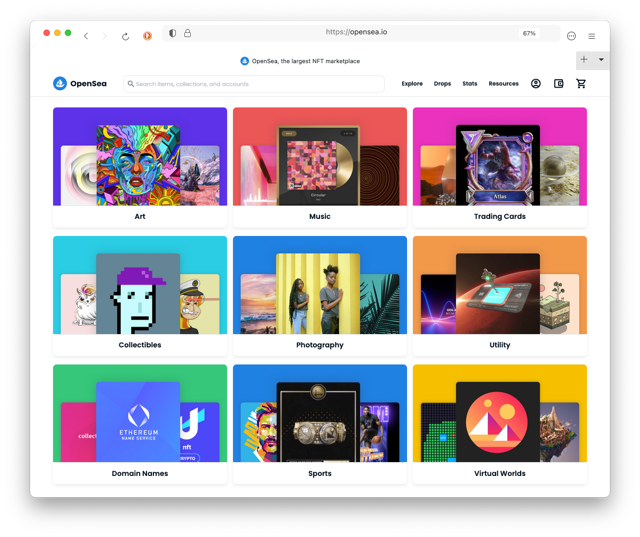
\includegraphics[width=.75\linewidth]{03-theory/opensea2022_1.png}
    \captionsetup{justification=centering,margin=1.5cm}
    \caption{Categories of NFTs being sold on one of the largest NFT marketplaces \citep[from][]{opensea2022a}}\label{fig: opensea2022_1}
\end{figure}

More recently, there are facets of the rise of NFT art projects that epitomise this continued fetishisation and veneration of digital fine art under the guise of `decentralisation'. Unfortunately enough, these projects often fall foul to the exact `centralisation' they market to oppose, creating small micro-communities of inter-centralised followers that collectively and actively, through social media, ensnare new and uninitiated retail investors via the urgency phenomenon of the `fear of missing out'. The motivation being to increase the value of their own NFTs - sometimes referred to as `shilling'. In most NFT projects, the only drive is profit motive, the digital art is merely the vehicle through which this investment is (im)materially realised. Despite the technological basis of some of these projects being quite radical in their proposition of democratic ownership and the privacy and security of digital information through decentralisation, the asset class most of them end up facilitating is tied to a a method of procurement and self-promotion that necessitates the enrichment of the creators and early adopters of that specific NFT collection. How, in any way, could this method of production and consumption be said to be different from Dewey's outlining of the rise of the `nouveaux riches':
\begin{quote}
    `The nouveaux riches, who are an important by-product of the capitalist system, have felt especially bound to surround themselves with works of fine art which, being rare, are also costly. Generally speaking, the typical collector is the typical capitalist. For evidence of good standing in the realm of higher culture, he amasses paintings, statuary, and artistic bijoux, as his stocks and bonds certify to his standing in the economic world.' \citeyearpar[p. 7]{dewey1934}
\end{quote}
It could be argued therefore, that we have witnessed an increase in the amount of new media formats, but not one that resituates production outside of capitalist logic for the masses; even in so called `decentralised' projects. When Leddy and Puolakka stress that it is this `private control of [the] forces of production for private gain' that leads to this disconnection of art from experience, it follows that the creation of art outside of the confines of this control addresses the imperative for the drawing of art `from all sources' [own emphasis]. From this view, the convergence of digital art to their `conditions of origin and operation in experience' could be seen as one of the primary foci of more recent movements such as Maker, Hacker, and DIY Labs, as well as the general ethos of participatory design and open-source hardware and software in art, design, and electronic music practice.

But what does it mean to say that art ought to originate and operate `in' experience, and how might these movements address this? Dewey considers the `live creature' in response to this question. He views the participant of aesthetic experience as meaningfully inseparable from the environment in which they are embedded: 
\begin{quote}
    `The senses are the organs through which the live creature participates directly in the on-goings of the world about [them]. In this participation the varied wonder and splendour of this world are made actual for [them] in the qualities [they experience]. This material cannot be opposed to action, for motor apparatus and `will' itself are the means by which this participation is carried on and directed. It cannot be opposed to `intellect', for mind is the means by which participation is rendered fruitful through sense; by which meanings and values are extracted, retained, and put to further service in the intercourse of the live creature with [their] surroundings.' \citeyearpar[p. 22]{dewey1934}
\end{quote}
From this basis, namely that perception, sensorimotor action, and intellect cannot be meaningfully separated when considering the intercourse of participants with their environment, Dewey highlights the weakness in the traditional dualist theory of mind - we are embodied and embedded beings. He posits that experience results from the `interaction of organism and environment',  and that in its fullest, experience can represent a `transformation of interaction into participation and communication'. It would follow, therefore, that in the production of artistic works, consideration of this dynamical relationship that constitutes our subjective experiences is not only valuable, but that artistic works should aim to arise (originate) from common and relatable states of this relationship. Returning art to this origination and operation `in' experience through interactive and participatory digital means can therefore be seen as a crucial mechanism for inducing positive societal change through fostering new channels of `participation and communication'. Shifting the production of artistic work away from the exploitative practices of mass manufacturing inherent in consumer technologies, as well as centring embodied participatory design practices, is a common theme among DIY and Makerspace communities.

This is not to in any way demean or reduce the social importance of art that does not take these approaches. It is also especially tricky to prove in any certainty the subjective measures of aesthetic experience that could result in positive societal change. However, I do view the imperative to shift production and consumption of art outside the capitalist architecture of current proprietary software tools and consumer technologies, and bringing the aesthetic closer to every day experience as a fruitful endeavour for the artist. I argue that doing so would emphasise the dynamical relationship participants find themselves in with their and, crucially, others' sociocultural, economic, and ecological contexts.

Where does knowledge lie for us as researchers in the production and consumption of such artistic works? On what basis can we test and evaluate these claims? One view that is popular in the field of music technology is that of considering the nature of the interactive and digital systems that we develop; a consideration of the epistemic tool. 
\begin{quote}
    `The digital instrument is an artefact primarily based on rational foundations, and, as a tool yielding hermeneutic relations, it is characterised by its origins in a specific culture. This portrayal highlights the strengthened responsibilities on the designers of digital tools, in terms of aesthetics and cultural influence, as they are more symbolic and of compositional pertinence than our physical tools.' \citep[p. 335]{magnusson2009a} 
\end{quote}

Developed by Magnusson, this line of thinking proposes that the digital instruments we design and employ as artists have inscribed in their physicality, affordance and sonic output, knowledge of cultural, historical, and designerly significance. In this way, they can be considered complex systems of research importance through the examination of their symbolic design, construction, performance, and appreciation by audiences. Magnusson embeds this proposition within Don Ihde's philosophy of `instrumental realism' and Wittgenstinian philosophy, and draws from an understanding of the extended mind hypothesis. This theory, which will be expanded on in the next section, proposes that 
\begin{quote}
    `[Under certain conditions], the human organism is linked with an external entity in a two-way interaction, creating a coupled system that can be seen as a cognitive system in its own right.' \citep[p. 7]{clark1998}
\end{quote}


Similar to Dewey's conception of how the live creature is inseparable from the environmental conditions that it is embedded in, the extended mind hypothesis and similar theories of embodied cognition prove to be invaluable in the field of tangible user interfaces, and digital music instrument design, due to the way they can explicate as well as draw out the dynamic relationships between artist, collaborator, material, interface, and audience in the deployment of expressive artistic media. In the following sections, I shall dive deeper into these theories of mind (ToM), and what they have to offer a practice that makes use of augmented reality technologies within the field of computational art and musical performance.

\begin{figure}[h]
    \centering
    \includegraphics[width=1\linewidth]{03-theory/úlfarsson2014.png}
    \captionsetup{justification=centering,margin=1.5cm}
    \caption{An early Halldorophone (cello-like feedback instrument) \citep[from][]{ulfarsson2014}}\label{fig: ulfarsson2014}
\end{figure}

% --------------------------------------------------------------------------- %
\section{The 4E Approach to Experience}\label{sec: theory-4e}
One way of expanding on this conception of aesthetic experience is to adopt the 4E approach to cognition and experience. Key to my following theoretical underpinning of materiality, embodiment, and space will involve how this approaches the themes of perception, agency and cognition arising through the complex inter-threaded coupling between a participant and their environment. Often referred to as `the 4 E's', 4E cognition (4EC), states that cognition is an embodied, embedded, enactive, and extended process \citep{gallagher2017}. It's worth mentioning that 4EC is an amalgam of related theories of mind (ToM) across the disciplines of philosophy and the social and cognitive sciences, and as such there are different flavours of it. Many of these have said to have roots in the Dewey's (among others') pragmatism outlined in the previous section, as well as Merleau-Ponty's embodiment theories \citep{zavota2016}. What these constituent theories all bear in common is the rejection of the standard cognitivist model of experience that states that cognitive processes happen solely `in the mind' and 'in the brain'. Another principle is that they generally draw from complex systems theory: `understanding the complex interplay of brain, body and world requires the tools and methods of nonlinear dynamical systems theory' \citep{clark1999}. Before delving into the specification and implications of a 4EC approach, I would first like to touch on this concept of complexity, as it will surface throughout the thesis. Within certain systems, which are deemed to be `complex', this field proposes that there are a multitude of phenomena that can explicate the interactions between components of such a continually unfolding system, including \citep{dedomenico2019}:
\begin{itemize}
    \item Interactions - a complex system is formed of many components, many of which will be connected in a network of mutual and on-going interaction
    \item Emergence - from this network of interactions, there exists the possibility for complex and novel structures to form that are inexplicable from the features of their simpler components 
    \item Dynamics - the state of a complex system can change over time, often in an unpredictable non-linear fashion
    \item Self-organisation - the components of a complex system may exhibit collective behaviours, and perceived large scale structure
    \item Adaptation - complex systems don't necessarily shift between steady states, they actively and reactively respond to environmental stimuli
    \item Feedback - structures of a complex system exhibit a phenomena where the outputs of a system are routed back in, via closed chains of cause and effect 
\end{itemize}

\begin{figure}[ht]
    \centering
    
\includegraphics[width=.65\linewidth]{03-theory/kentish2020.png}
    \captionsetup{justification=centering,margin=1.5cm}
    \caption{Starling murmuration displaying complex and emergent flocking behaviours \citep[taken by][in Brighton, UK]{kentish2020}}\label{fig: kentish2020}
\end{figure}

%% !!! check here, ben white
Thus, 4EC normally begins with an acknowledgement of the complex embodied nature of human cognition. Varela, Thompson, and Rosch propose that cognition is embodied in a way not too dissimilar to the assertion Dewey holds in regards to the `senses' of the `live creature'.
\begin{quote}
    `By using the term embodied we mean to highlight two points: first, that cognition depends upon the kinds of experience that come from having a body with various sensorimotor capacities, and second, that these individual sensorimotor capacities are themselves embedded in a more encompassing biological, psychological, and cultural context.' \citeyearpar[pp. 172-173]{varela1993}
\end{quote}
Alva Nöe's concept of sensorimotor contingencies has since built on the first point of this approach to embodiment, in a way that proposes an `enactive approach to perception' accepts that perception is something we do, not something that happens to us \citep{noe2004}. This has since been termed the `sensorimotor approach' to enactivism, and Gallagher notes that it falls short of an `enactivist approach' due to its omission of affective aspects of embodiment such as `mood-related and emotional factors, […] bodily states such as hunger, fatigue, and pain, as well as a complex motivational dimension that animates body-world interaction' \citep[p. 150]{gallagher2017} The proposal is that that an `enactivist' approach, i.e. one that aligns with Varela, Thompson, and Rosch's claim that sensorimotor capacity is `embedded in biological, psychological, and cultural contexts' more holistic perspective, the proponents of embodiment theories of 4EC propose a radical shift from the standard cognitivist ToM; sensory perception and bodily existence is not only causally related to the emergence of cognitive processes, it literally constitutes them. 

A natural continuation extends this line of reasoning to the material environment in which the participant is a part of — accepting that it is in turn shaped by the web of sociocultural norms and values that Dewey alludes to, and is the site of sensorimotor action. Mark Rowlands proposes this underlying thesis as `the embedded mind':
\begin{quote}
    `In accomplishing cognitive tasks, an organism can utilize structures in its environment in such a way that the amount of internal processing it must perform is reduced. Some of the complexity of the task is, thereby, off-loaded onto the environment, given that the organism has the ability to appropriately exploit that environment.' \citeyearpar[p. 68]{rowlands2010}  
\end{quote}
It necessarily follows that if a cognitive system that has the potential for environmentally embedded sensorimotor action, i.e. it is embodied and embedded, it also enacts its cognition. The first formal account of what could be called an enactive approach to cognition begins also in `The Embodied Mind', by Varela, Thompson and Rosch. From a foundation of accepting that sensory and motor processes, namely perception and action, are `inseparable in lived cognition', enaction is contingent on two assumptions: perception consists in perceptually guided action, and cognitive structures emerge from the recurrent sensorimotor patterns that enable action to be perceptually guided \citeyearpar[p. 173]{varela1993}. The authors argue that an enactive approach to cognition therefore proposes that perception must be studied from the point of view of the participant's sensorimotor structure, rather than any `pre-given, perceiver-dependent world', i.e. the world is not perceived through an internal representational model of what is `outside', rather, the world emerges from a participants ability to `guide [their] actions in [their] local situation', to enact.

The last assertion of a 4EC account claims that cognition has the potential to be extended into objects in a participants environment. The extended mind hypothesis, as developed by Andy Clark and David Chalmers and described in the previous section, is the core thesis of this proposal. The authors propose that, cognitive processes, beliefs for example, can be `constituted partly by features in the environment, when those features play the right sort of role in driving cognitive processes' \citeyearpar[p. 12]{clark1998}. They compare the experience of cognition in two different hypothetical people, Inga and Otto. Both are tasked with recalling the address of a museum and travelling to it. Inga has a neurotypically functioning memory, and so accesses the memory of the address (which assumedly lay dormant previous to this action) recalls it, and travels to the address. Otto has Alzheimers, and like many others with Alzheimers relies on the use of a notebook or memory aid to recall experiences and other important information, he finds the address in the notebook, and travels to the museum. In both cases, Clark and Chalmers propose that the cognitive functionality of what constitutes 'belief' are analogous:
\begin{quote}
    `To say that the beliefs disappear when the notebook is filed away seems to miss the big picture in just the same way as saying that Inga's beliefs disappear as soon as she is [no] longer conscious of them. In both cases the information is reliably there when needed, available to consciousness and available to guide action, just the way that we expect a belief to be' \citeyearpar[13]{clark1998}.
\end{quote}

\begin{figure}[ht]
    \centering
    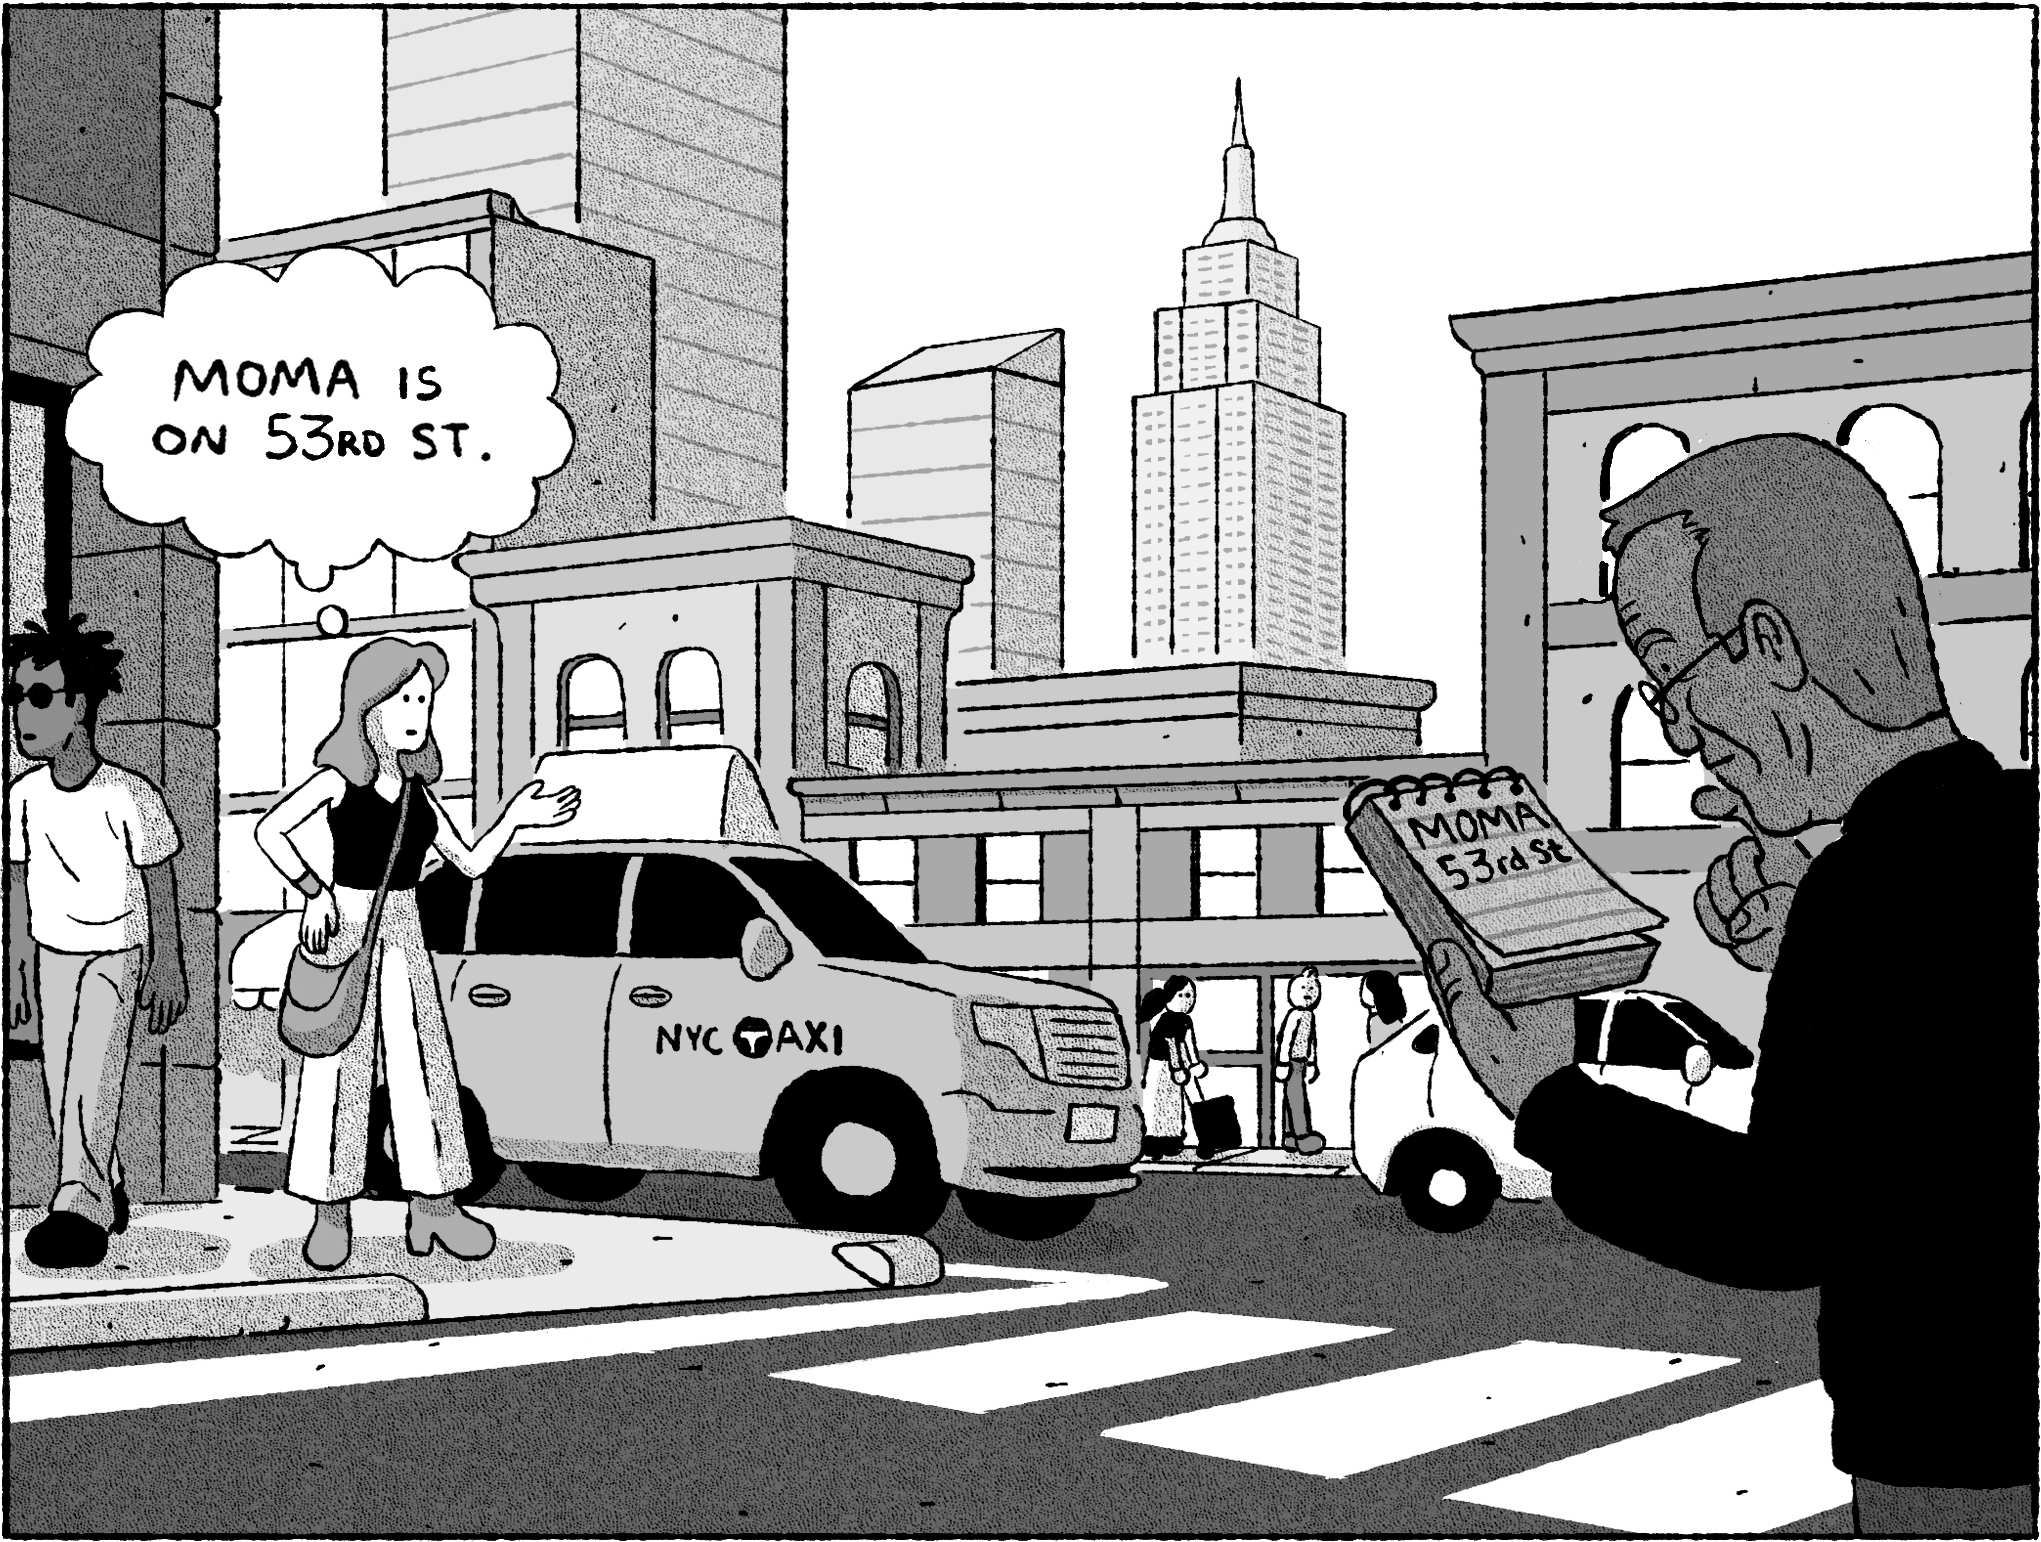
\includegraphics[width=.75\linewidth]{03-theory/chalmers2022_1.png}
    \captionsetup{justification=centering,margin=1.5cm}
    \caption{Inga and Otto on their way to the MoMA \citep[by Tim Peacock in][]{chalmers2022}}\label{fig: chalmers2022_1}
\end{figure}

It therefore follows, that cognition is extended, beyond the boundary of the mind-body and into the environment, and even into specific artefacts - a key theory that enables the proposition of Magnusson's epistemic tool within the field of music technology, as mentioned previously. Taking these four points of departure, namely that cognition is embodied, embedded, enacted, and extended, Gallagher presents the following assumptions as the core conditions of an enactivist approach to cognition \citep[p. 6]{gallagher2017}:
\begin{enumerate}
    \item Cognition is not simply a brain event. It emerges from processes distributed across brain – body – environment. The mind is embodied; from a first-person perspective embodiment is equivalent to the phenomenological concept of the lived body. From a third-person perspective the organism–environment is taken as the explanatory unit.
    \item The world (meaning, intentionality) is not pre-given or predefined, but is structured by cognition and action
    \item Cognitive processes acquire meaning in part by their role in the context of action, rather than through a representational mapping or replicated internal model of the world
    \item Enactivist approaches have strong links to dynamical systems theory, emphasising the relevance of dynamical coupling and coordination across brain – body – environment
    \item In contrast to classic cognitive science, which is often characterised by methodological individualism with a focus on internal mechanisms, enactivist approaches emphasize the extended, intersubjective, and socially situated nature of cognitive systems. Enactivism aims to ground higher and more complex cognitive functions not only in sensorimotor coordination, but also in affective and autonomic aspects of the full body.
    \item Higher-order cognitive functions, such as reflective thinking or deliberation, are exercises of skilful know-how and are usually coupled with situated and embodied actions
\end{enumerate}
Poignantly, this way of framing our human experience is salient for the digital humanities at this point in time. More of our everyday social, artistic, political, cultural, environmental, and economic interactions are mediated by technologies and platforms. These are privately owned by mega-corporations, that as previously mentioned, have shown dubious a relationship with ethics concerning misinformation and user privacy, as well as extractivist methods of guaranteeing shareholder profit. Does Facebook's `metaverse' sound like the kind of \gls{ar} environment that sounds like a safe and democratic ground for art that seeks the `transformation of interaction into participation and communication' \citep[]{dewey1934}? This decision is up to the reader, but I would argue not as it will become clear in the following sections.

Out of this model of explicating experience, I propose three lenses through which to examine \gls{ar} applications in the sonic arts - materiality, embodiment, and spatiality. In some ways, a linear, written account of these processes, separated neatly by subheadings is somewhat incompatible with the logic of 4EC and its process-inseparability, nevertheless, in the following sections of this chapter I will attempt to go into detail how we can use this model of experience, to consider the themes of materiality, embodiment, and space within \gls{ar} musical instrument research practice, as well as the broader study of digital humanities. Loosely, these three sections will cover the artistic, audience, and societal considerations and potentialities respectively, when engaging with \gls{ar} systems.



% --------------------------------------------------------------------------- %
\section{Complex Material in Interactive Music Systems}\label{sec: theory-materiality}
Thus far, we have outlined the contextual origins of \gls{ar} technology, as well as their contemporary physical forms, modes of sensory display, and methods of real and virtual processing. Additionally, I have outlined the theories of aesthetic and perceptual experience through which these technologies could be interrogated to further understand \gls{ar}'s role as a medium for artistic expression. In this section I will propose a lens through which to consider the artist's composition of `material' in \gls{ar} experiences as a method of fostering a modulated dialogue between elements of a participants sensorimotor engagement with their perceived real and virtual environment. 

Existing frameworks for considering the design of relationships between real and virtual processes do exist within in the field of \gls{ar}; in the early 90's, the theoretical work of Milgram and Kishino, their reality-virtuality continuum \citeyearpar[p. 10]{milgram1994}, proved to be a fruitful way of sorting the types of \gls{ar} and VR technologies that were arising from different fields at the time. However, for my purposes of detailing the material nature of an artists' composition in \gls{ar}, a more nuanced and detailed framework is needed, one that goes beyond specifying the what (a spectrum of reality to virtuality); towards a investigating of the how, (a processual space of augmentation, diminution, alteration, hybridisation, and extension through which real and virtual environments are enmeshed), and the why (the conveyance of meaning and intentionality of the artistic work). 

Hanna Schraffenberger, as highlighted in \autoref{sec: ar-process}, offers a set of relations that describe the dynamics between `the virtual and the real' (see \autoref{table:schraffenbergertaxonomy}, \pageref{table:schraffenbergertaxonomy}). She argues that from the fundamental relationships of presence, information, physicality, and behaviour, there emerge new `subforms' of \gls{ar}, namely extended, diminished, altered and hybrid reality, as well as extended perception. Yet, even with this level of description, the processes themselves are still abstract - these are descriptors for the types of processes, but what are the processes themselves? I believe that the answer lies again, in an approach aligned with complex systems theory; through a consideration of phenomena such as interaction, emergence, dynamics, self-organisation, adaptation, and feedback.

\begin{wrapfigure}{r}{0.45\textwidth}
    \vspace{-\intextsep}
    \hfill
    \begin{minipage}{0.95\linewidth}
        
\includegraphics[width=\linewidth]{03-theory/delaney2017.png}
        \captionsetup{justification=justified}
        \caption{Atau Tanaka performing \textit{Myogram}, an 8 channel sonification of muscular corporeal states \citep[taken by][]{delaney2017}}\label{fig: delaney2017}
    \end{minipage}
\end{wrapfigure}

Within the field of music interfaces, considerable research and practice has been conducted in the area of complex systems. Surmised neatly by musical interface researcher Joel Ryan, hidden, or black-boxed complex processes within digital interfaces can be developed and explored through ascribing `physical handles' to these `phantom models', e.g. providing embodied interaction to algorithmic musical processes to better understand, design, and evaluate them.
\begin{quote}
    `The physicality of the performance interface helps give definition to the modelling process itself. The physical relation to a model stimulates the imagination and enables the elaboration of the model using spatial and physical metaphors. The image with which the artist works to realise his or her idea is no longer a phantom, it can be touched, navigated and negotiated with.' \citeyearpar[p.5]{ryan1991}
\end{quote}
Perhaps the design of \gls{ar} musical instruments is concerned with not only providing physical handles to phantom models, but phantom handles to physical models too.

In the same vein, Agostino Di Scipio outlined his perspective on the paradigm of interaction in the context of audio signal processing and musical interface use. 
\begin{quote}
    `Interactive music systems are dedicated computational tools capable of reacting in real time, upon changes in their `external conditions', [typically including] initial input data and run-time control data […] set, changed and adjusted by some agent – a performer, or group of performers […] Control devices, with their mechanical and/or visual interfaces, are operated to determine these data.\\ 

    The main purpose of control data is to determine a system's changes of internal state. This is done indirectly, by updating the parameters in either digital signal processing techniques or program routines operating at a more abstract, symbolic level. Changes of internal state are heard as changes in the musical output. By operating the available control devices, the agent in effect `plays' the system as if it were a new kind of music instrument' \citeyearpar[p. 1]{discipio2003}
\end{quote}
For Di Scipio, the act of integrating the agent / performer into the definition of the music system implies that 'interaction' exists in the `underlying ontology' or `interdependent coupling' of participant and instrument; at the site of their `interface'. This coupling creates linear feedback loops in performance, between the resultant sound, and decisions made by the performer. Indeed, this lower-level dependency (human-machine) itself exists within the wider `meta-system' including `[human], machine and environment'. Within this meta-system, later referred to as an `ecosystem', Di Scipio outlines that:
\begin{quote}
    `A principal aim would be to create a dynamical system exhibiting an adaptive behaviour to the surrounding external conditions, and capable to interfere with the external conditions themselves. Not only would it be able to detect changes in the external world and `hear' what happens out there, […] it would also be able to become a self-observing system, that is, to determine its own internal states based on the available information on the external conditions – including the traces of its own existence left in the surroundings. […] This [move towards composing musical interactions] should be described as a shift from creating wanted sounds via interactive means, towards creating wanted interactions having audible traces. In the latter case, one designs, implements and maintains a network of connected components whose emergent behaviour in sound one calls music.' \citeyearpar[p. 6]{discipio2003}
\end{quote}

\begin{wrapfigure}{l}{0.45\textwidth}
    \begin{minipage}{0.95\linewidth}
        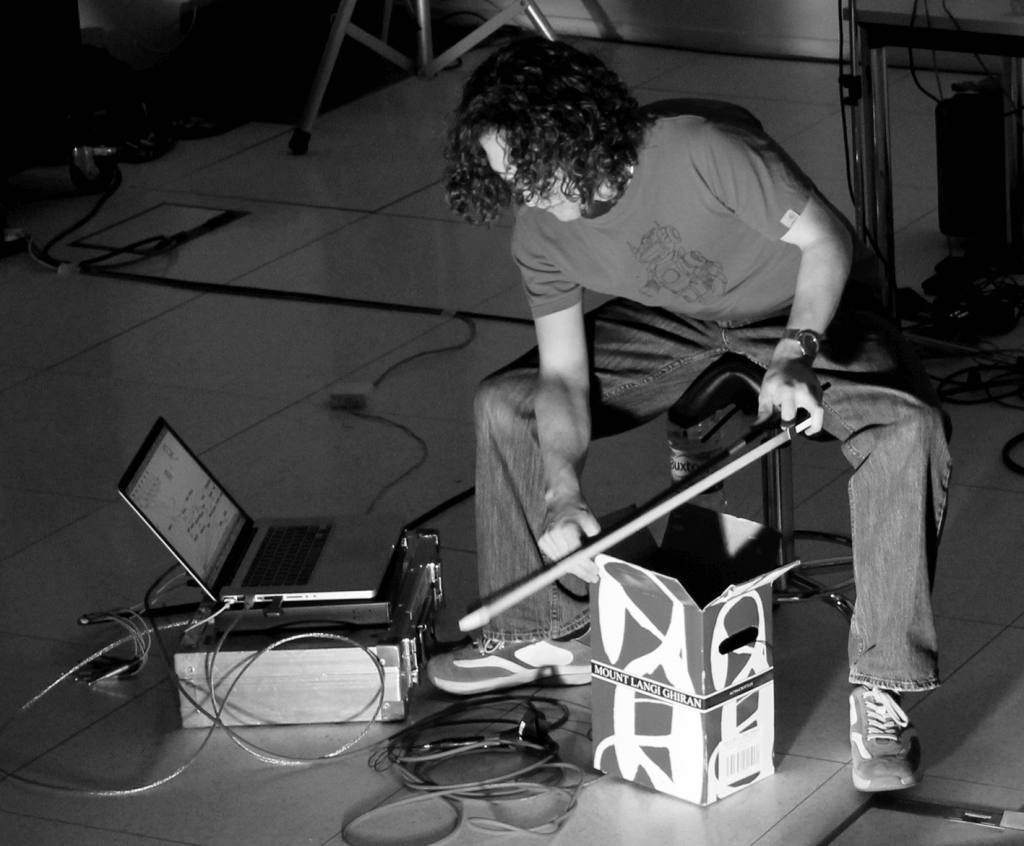
\includegraphics[width=\linewidth]{03-theory/green2010.png}
        \captionsetup{justification=justified}
        \caption{Bowed Cardboard Box in performance \textit{Cardboard Cutout} \citep[from][]{green2010}}
    \end{minipage}
    \hfill
\end{wrapfigure}

The depth of research based on this type of complex interactive music system (IMS) has deepened considerably in the last 20 years, as artificial intelligence and machine learning algorithms, low-latency microcontrollers, and real-time compositional software have been implemented into what Magnusson terms `intelligent instruments' \citeyearpar[p. 8]{magnusson2009}. Thus, `performative ecosystems' \citep[]{waters2007} such as these exhibit behaviours of complex systems as mentioned above, including interaction, emergence, dynamics, self-organisation, adaptation, and feedback. I propose therefore that an enactivist approach to experience (4EC), one that posits the emergence of cognitive processes across the distributed system of mind-body-environment as being wholly appropriate in the design, creation, performance, an evaluation of interactive music ecosystems. 

Some of the first proponents of this approach include Essl and O'Modhrain, who propose an enactive approach they term `weak sensorimotor integration' to the design philosophy of tangible interfaces for musical expression. `What concerns us here[…], is the consideration of enactive knowledge in the context of musical instrument design and how perceptually guided action defines the `feel' and playability of a musical instrument.' \citeyearpar[p. 3]{essl2006}. Core to their research is the question: `In what way does a specific integration of sensory perception and motor action correspond to a controllable, even enjoyable musical performance experience?' Building on the class of expected sounds that correlate to our action with physical objects in the world, Essl and O'Modhrain evaluate the design of a set of prototype tangible interfaces that introduce a flexibility in this expectation-realisation coupling between action and sound by altering the digital sonic output of the system based on measured user interaction. They propose that the resultant interaction with these instruments provided grounds to include a loose sensorimotor integration into the design of musical interfaces. The present thesis is interested in the implication of this hypothesis in the creation of not only physical interactions with IMS, but also virtual, and ultimately, hybrid interactions. My own 4EC approach to the compositional material of \gls{ar} musical experiences draws from Essl and O'Modhrain's own motivation for their proposal of an enactive approach. How are dynamics of \gls{ar} musical systems learnt over time? How is the ability to predict musical outcomes affected by the integration real-time motion sensing and parameter mapping? How does the configuration of hybrid sensory content define the way action becomes perceptually guided?

Newton Armstrong also provides considerable insight on the enactive design of DMIs. He proposes an `enactive model of interaction' that is concerned with `circular chains of embodied interdependency between performer and instrument, instrumental `resistance' to human action and intentionality, and an integrative approach to the roles of sensing, acting and cognitive process in the incremental acquisition of performative skill.' For Armstrong, this approach draws from a principled distinction between `functional' and `realizational' interfaces. Whereas a functional interface `serves a predetermined function; it is structured around a finite set of interactions which are known in advance of the task's execution', a realizational interface `brings with it the possibility of continuously realizing new encounters and uses, and, in the process, of re-determining the relationship between technical objects and their human subjects' \citep[p. v]{armstrong2006}. This distinction, and a pursuit of the latter over the former, means to prioritise the contexts of `meaning and signification in which human and medium are embedded, and is conducive to dynamic and indeterminate forms of interaction' (p.42). These dynamic forms of interaction are realised through performer intention, and instrumental `resistance' in response the performer's engagement with it. Over time, this resistance establishes adaptation in participant interaction, constituting what Armstrong terms a `dynamical responsiveness' between the performer and their instrument (pp.46-47). 

\begin{wrapfigure}{r}{0.45\textwidth}
    \vspace{-\intextsep}
    \hfill
    \begin{minipage}{0.95\linewidth}
        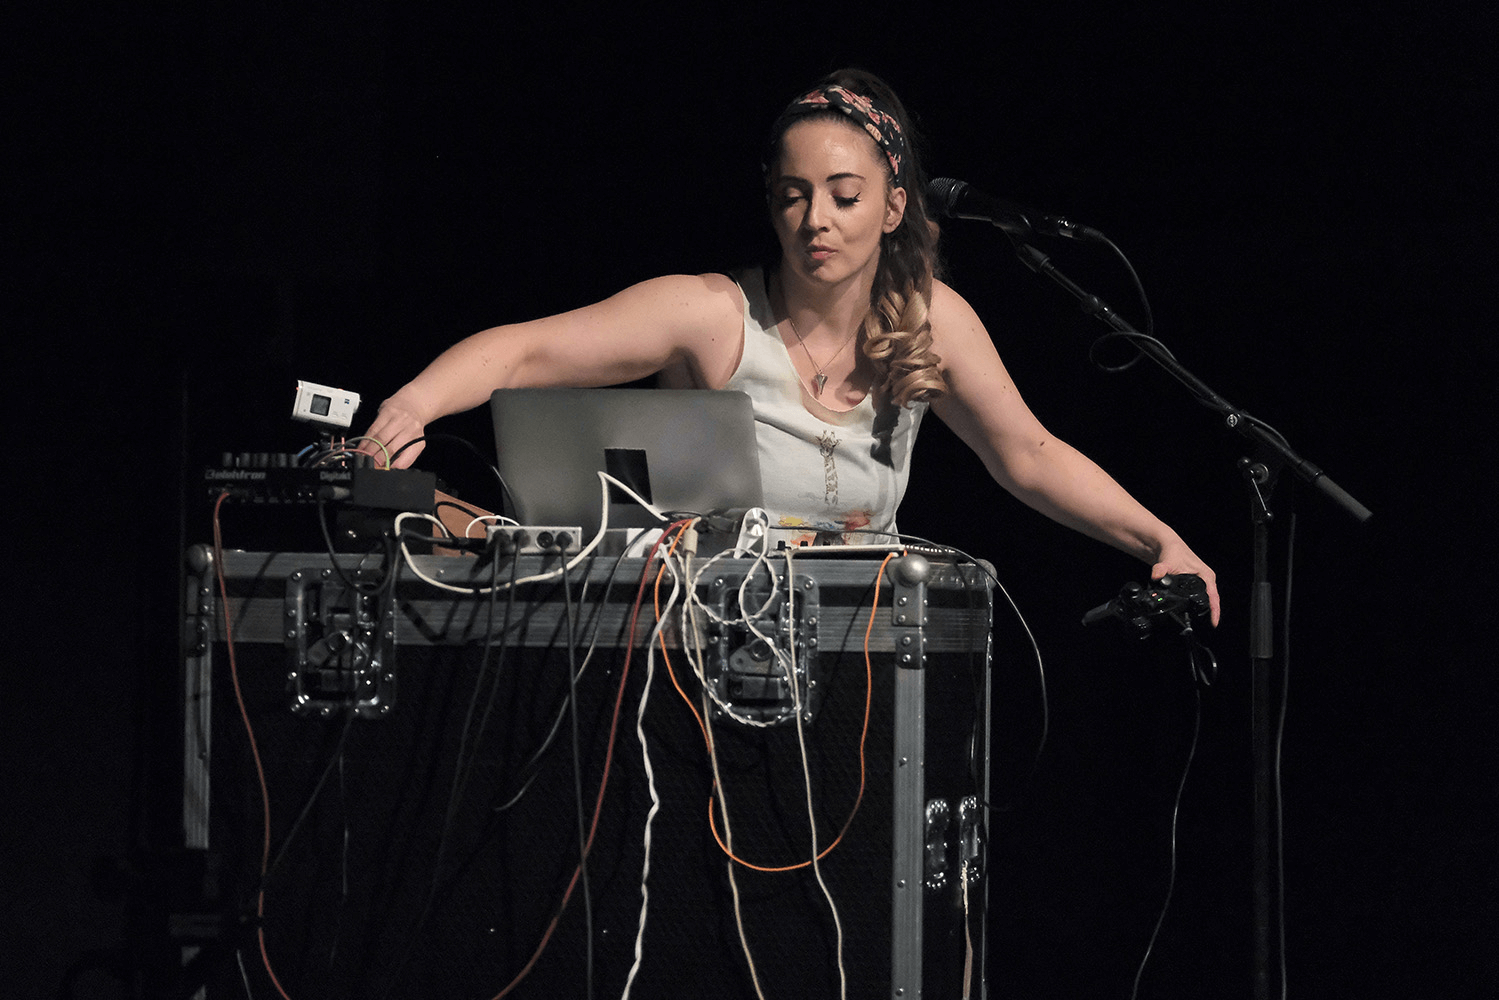
\includegraphics[width=\linewidth]{03-theory/hayes2019.png}
        \captionsetup{justification=justified}
        \caption{\textit{Moon via Spirit} by Lauren Sarah Hayes in performance \citep[taken by][]{slater2019}}\label{fig: slater2019}
    \end{minipage}
\end{wrapfigure}

Lauren Sarah Hayes' work approaches live electronic music practice from an enactive and embodied perspective. This work often uses tangible and haptic controllers that provide non-linear controller input to various elements of the `ecological network of sound analysis and digital signal processing' that constitutes her performance ecosystems. For Hayes, designing complex and adaptive musical systems allows `elements of instability, vulnerability, unpredictability [to] become fodder for the improviser' \citep[p. 2]{hayes2018}. Hayes' creative and research practice has enabled a pedagogical methodology, in which `music and movement-based improvisational practices' are explored in classes of undergraduate students. Through a combination of deep listening methods, movement exercises, and free improvisational exercises, Hayes argues that there is a potential for co-creation of compelling improvisational performances in classes of up to thirty untrained improvisers. These techniques result not only in the active exploration of musical sensorimotor contingencies, but also in the creation of musical meaning that is `brought forth through an emergent extended cognitive network that involves complex relationships between the improvisers involved, technology, and the space in which the performer-instrument pairings are distributed' \citep[p. 8]{hayes2019}. These ensemble improvisations draw from a wide variety of media formats including \gls{ar}. Pointing towards the following assertion by Schiavio and van der Schyff \citeyearpar{schiavio2018}, Hayes notes that digital musical instrument practice ought to develop and augment improvisational practices `that build collectively on individual musical and creative sociocultural histories that individuals bring to the table':
\begin{quote}
    `If the body plays a key role in determining musical learning, so does the socio-material and cultural environment in which it is embedded. However, these dimensions are not separated from the body. Rather, they become manifest through the body and are co-determined by actions and interactions with other bodies and things in socio-culturally meaningful contexts.` \citep[p. 9]{hayes2018}
\end{quote}

\begin{wrapfigure}{l}{0.45\textwidth}
    \vspace{-\intextsep}
\begin{minipage}{0.95\linewidth}
    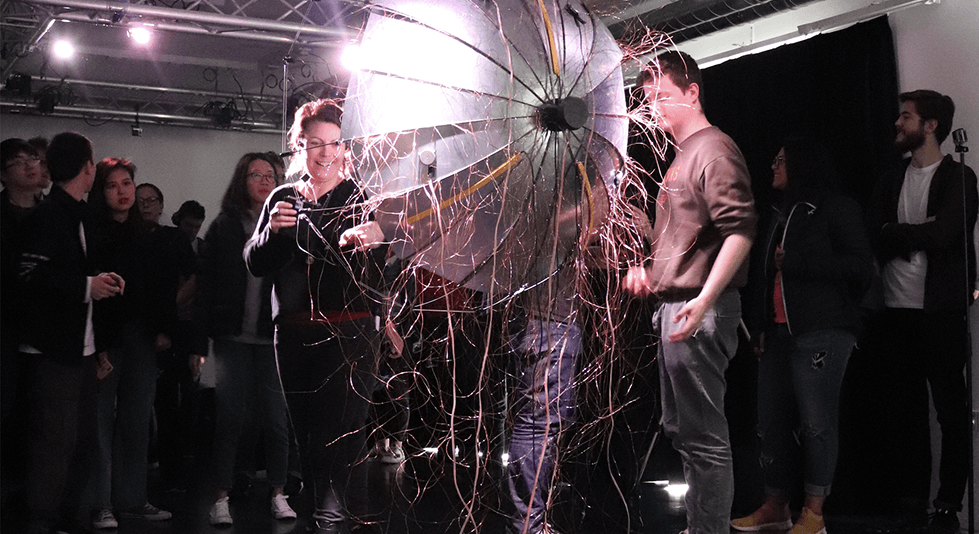
\includegraphics[width=\linewidth]{03-theory/chevalier2019.png}
    \captionsetup{justification=justified}
    \caption{Multiple participants engage with Listening Mirrors \citep[from][]{chevalier2019}}\label{fig: chevalier2019}
\end{minipage}
\hfill
\end{wrapfigure}

Chevalier and Kiefer propose a similar method of promoting musical expression in their \gls{aar} work `Listening Mirrors' \citeyearpar[]{chevalier2018}. Their is system is `audience participation dependent`, and could constitute a realisational DMI. Through real-time analysis and re-projection of participants' breath and vocal sounds via bone-conduction headphones and a transducer-augmented parabolic mirror, audience members, environment, and interfaces `feed off each other`, co-creating physical and virtual sound environments that overlap and co-construct a shared hybrid listening space. Their creative and research practice is situated in the later work of Merleau-Ponty and related theories of enactivism. In particular, Chevalier draws from Merleau-Ponty's notion of the `flesh':
\begin{quote}
    `In defining what is meant by `flesh', Merleau-Ponty states, `[w]e must seek space and its content together', that we are `interwoven into a single fabric', a `universal flesh', and `he who sees cannot possess the visible unless he is possessed by it, unless he is of it'. The notion of `flesh', therefore, is both the `flesh of the world' and the `flesh of the body', the relation of the corps sauvage and cultural world and its representations.' (\citeauthor[p. 58]{chevalier2016}, \citeyearpar{chevalier2016}  citing \citeauthor{merleau-ponty1945}, \citeyearpar{merleau-ponty1945,merleau-ponty1968})
\end{quote}

Thus, depending on the specific artwork, from any or each of the DMI designer's \citep[]{essl2006,armstrong2006}, improvisational performer's \citep[]{hayes2019}, or installation artist's \citep[]{chevalier2018} perspective, if the material composition of the system with which they are engaging is designed to provide a realisational, dynamic interaction then it `assumes open-ended, fluid, and at least partly indeterminate processes of signification, and as such requires the ongoing cognitive involvement of the musician' \citep[p. 48]{armstrong2006}. This necessity of engagement aesthetically situates such artworks and instruments closer to the site of everyday embodied life, what Dewey terms the return of art to its `origin and operation' in experience. These examples also align themselves with the 4EC approach to experience, which argues that cognitive process are embodied, embedded, enacted, and extended, across a distribution of mind - body - environment. 

Augmented reality, specifically due to its ability to mediate perception in real-time and across a multitude of sensory modalities, presents the opportunity to `experiment with, modulate and disrupt [conditions of situated-ness, timeliness, emergence, multimodality and engagement inherent to our embodied coupling] to create new audience collective experiences' \citep[]{chevalier2018}



% --------------------------------------------------------------------------- %
\section{Enactivist Approaches to the Body in XR Systems}\label{sec: theory-embodiment}
We started this chapter with an examination of John Dewey's account of the separation of art from everyday life, and the effect on it thereof. To account for the notion of an aesthetic experience in the appreciation of artistic works, Dewey points towards the `live creature'. This concept, as discussed, contributed to the modern study of 4EC: the notion that cognitive processes ought to be thought of as embodied, embedded, enactive, and extended across the distribution of brain-body-environment. The previous section outlined my approach to material composition from an artists perspective. The medium of \gls{ar} may be thought of as an `invocation of a performance ecosystem constituted of relationships between real and virtual processes in the axes of spatial, thematic, material and ecological distance'. The present section moves forward to consider the experience of participants in such artworks.

%[ ] check \clearpage
\subsection{Embodiment and Enactivism in VR}\label{sec: theory-embodimentvr}
Considerable amounts of research related to embodiment in the context of virtual environments (VEs) generally falls under specific but necessary discussions and measurements of particular cognitive and affective processes such as presence, emotion, awareness, and consciousness \citep[]{slater1994,seth2012}, for example, in body swap experiments \citep[]{slater2010}, the rubber-hand illusion \citep[]{suzuki2013}, and stimulating altered visual phenomenology \citep[]{suzuki2017}, as shown in \autoref{fig: suzuki2017}. Integration of explicitly 4EC approaches to VEs/VR have only started to appear in research in the last 10 years, and is generally lacking from the discourse around \gls{ar}. For example, through an two and a half year autoethnographic exploration of her own experience in the popular VE Second Life, Maeva Veerapen integrated the phenomenological theories of Merleau-Ponty and Husserl to analyse and explicate the specific location of `embodiment' inherent in the connection to her virtual avatar. She surmised that `such an experience is still anchored within the user's physical body and that its relation with the avatar's body creates the link between the two spaces, physical and virtual' and termed this state of being symbembodiment - symbiotic embodiment of a combined real and virtual self \citep[]{veerapen2011}. 
\begin{wrapfigure}{r}{0.45\textwidth}
    \hfill
    \begin{minipage}{0.95\linewidth}
        \includegraphics[width=\linewidth]{03-theory/suzuki2017.png}
        \captionsetup{justification=justified}
        \caption{Google DeepDream providing (non-realtime) altered visual phenomenology of Sussex campus via VR playback \citep[from][]{suzuki2017a}}\label{fig: suzuki2017}
    \end{minipage}
\end{wrapfigure}

Drawing on Veerapen's notion of symbembodiment and linking it to an enactivist approach (indeed, as Varela, Thompson, and Rosch state in their `The Embodied Mind', Merleau-Ponty and Husserl's theories form part of the Western phenomenological roots of their approach \citeyearpar[pp. 173, 18]{varela1993}), Willans et al. argue that the `episodes of emotion' in the experience of VEs are linked with feelings of `presence', which in turn emerges from the embedded nature of a participants sensorimotor structure, or, we might say, enaction \citeyearpar[p. 23]{willans2016}. Hovhannisyan et al. argue for an enactivist approach to understanding participant flow, which is motivated by the authors' resistance to the physicalist approach to designing `object-centred'  VR experiences that is typically employed \citeyearpar[p. 1]{hovhannisyan2019}. In particular, they turn attention towards what they call an action-predicated perspective (one that focuses on the enactivist theory of perceptually guided action) that they state is `non-reductive with respect to subjective experience', and honours `the pragmatic dimension of perceptual reality' \citeyearpar[p. 18]{hovhannisyan2019}. 

\subsection{Embodiment and Enactivism in AR}\label{sec: theory-embodimentar}
Within \gls{ar}, Riva et al. propose that \gls{ar} and VR can transform our `external experience' through the increased levels of presence and engagement they afford, that in turn generates `personal efficacy and self-reflectiveness' \citeyearpar[p. 10]{riva2016}, they further propose that it has the potential to do the same for our `internal experience' . For the authors, `bodily self-consciousness' can be enhanced and extended by altering/extending its boundaries through a process called 'augmented embodiment' , which builds on the hypothesis that embodiment could be altered, expanded, and distributed through \gls{ar} technology: 
\begin{quote}
    `Whenever computer-based information is blended with the perception of the surrounding physical world, as in augmented reality this may become integrated into a new form of altered embodiment. But that requires that the augmentation of the physical with the virtual be carried out in such a way that the user has the potential to feel present. Given the clear popularity of mobility and social connectivity, it seems that presence will increasingly be experienced through attention to an external world in which the physical and the virtual are somehow blended' \citep[]{waterworth2014}
\end{quote}
From an 4EC approach, `feeling present' in the context of bodily `mobility and social connectivity', emerges, and could be seen to be somewhat analogous with, the notion of action (and other cognitive processes) being embedded in the  socio-cultural and -material norms and values of a participant's environment, their inherent sensorimotor embodiment, and as a result, the propensity for their actions to be perceptually guided (enaction). Suzuki et al. operationalise Nöe's \citeyearpar[]{noe2004} concept of sensorimotor contingencies, as further developed by Seth in the field of predictive processing \citeyearpar[]{seth2014}, by using \gls{ar}/VR technology as a test-bed for exploring the effect of modulated sensorimotor contingency and congruency in participant's visual experience of familiar and unfamiliar 3D objects \citep[]{suzuki2019}. Their results indicate that `that the contingency, but not the congruency, of a person's actions and their visual consequences influences access to visual awareness', providing support for a 4E-like perspective on perception (and also hinting at the ability for \gls{ar}/VR technology to be used as a method for purposeful sensory illusion through sensorimotor incongruence). Most recently, Chalmers has argued that \gls{ar} has the potential to extend our mind in a more seamless fashion, in a way that he likens to Heidegger's proposal of the `ready-to-hand' nature of certain tools; in use they become an extension of our body without our having to `think' about them and the actions they afford.
\begin{quote}
    `What sort of mental processes do augmented reality devices extend? For a start, they can more seamlessly extend all the processes that smartphones extend: memory (remembering someone's birthday), navigation (getting to the museum), decision-making (deciding where to eat), communication (talking to friends), language processing (translating from another language), and more. But their immersive connection to our perceptual system provides new avenues for extension' \citep[p. 299]{chalmers2022}
\end{quote}
Chalmers further proposes that \gls{ar} provides the grounds for further cognitive extension: our abilities of perception (e.g. through infra-red sensing), recognition (through algorithmic processing and machine learning of real-time environmental data), and imagination (through real-time replacement or transformation of physical objects with virtual ones). Considering Ishi and Omar, -- Inga and Otto's 21st century counterparts -- in \autoref{fig: chalmers2022_2}, Chalmers shows that \gls{ar} devices can theoretically provide cognitive extension, vis-a-vis `The Extended Mind'.

\begin{figure}[ht]
    \centering
    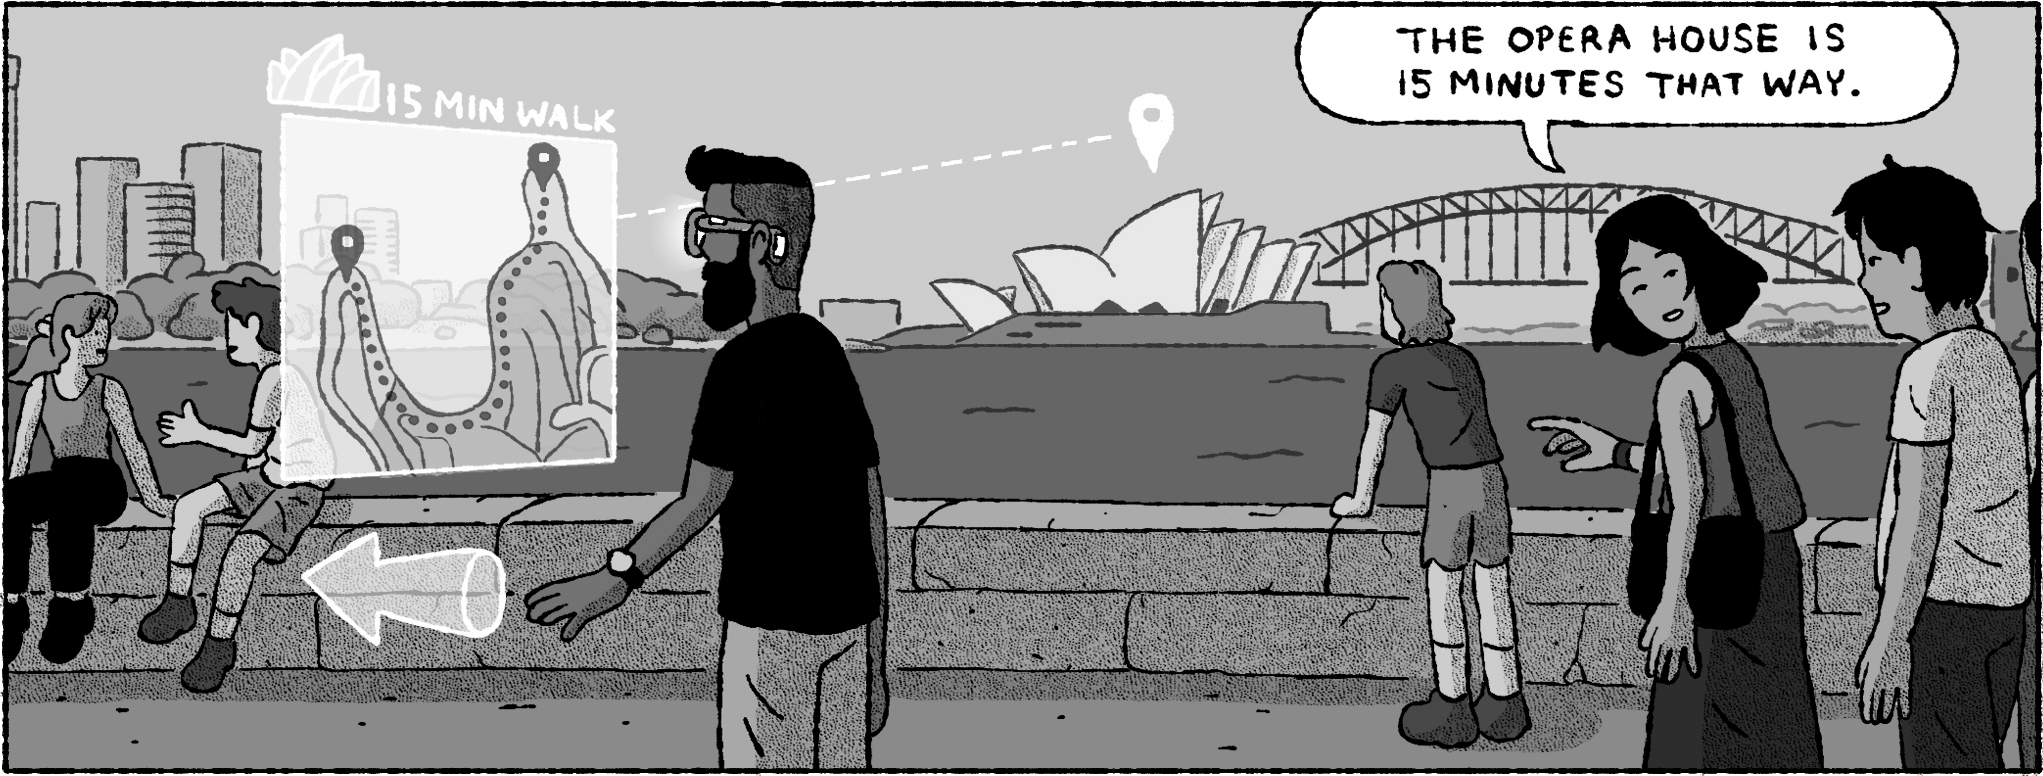
\includegraphics[width=1\linewidth]{03-theory/chalmers2022_2.png}
    \captionsetup{justification=centering,margin=1.5cm}
    \caption{Ishi and Omar on their individually recollected routes to the Sydney Opera House \citep[by Tim Peacock, in][]{chalmers2022}}\label{fig: chalmers2022_2}
\end{figure}



% --------------------------------------------------------------------------- %
\section{The Elephant in Our Headsets: The Zuckerverse}\label{sec: theory-space}
As we have established so far, \gls{ar}, when applied as a medium for the composition, performance, and expression of multisensory art and music, has the potential to:
\begin{enumerate}
    \item Provide new modes of instrumental performance and expression to performers and participants
    \item Radically modulate the embodied experience of performers and participants
    \item Scaffold new musical and artistic meaning through these augmented aesthetic experiences
\end{enumerate}
It follows that such experiences appropriate existing physically real spaces to do so, whilst either (a) simultaneously creating a relational virtual space dependent on the content of the experience, or (b) appropriating physically real spaces to the ends of constructing an entirely new hybrid \gls{ar} space that is greater than the sum of its physical and virtual counterparts. In current popular culture, this notion of a type of physical and virtual hybrid space has been given the term (the) `Metaverse'.

`The Metaverse' gained popularity as a term partway through this writing thesis, partly due to Facebook's calculated re-brand to Meta, partly due to the resulting `bull' run in `metaverse' cryptocurrencies, and partly due to the large subsequent increase of venture capital funding in XR start-ups. The reality is however that it is not a new term, having originated from Neal Stephenson's \textit{Snow Crash} \citep[]{stephenson1992}, a sci-fi novel detailing an anarcho-capitalist future in which a VR-based internet (The Metaverse) has become the gamified site of socio-cultural and economic norms, values, and interactions. In textit{Snow Crash}, Metaverse users immerse themselves via personal or publicly available terminals (see VR), although using public terminals has a negative affect on your avatar appearance and thus your status in The Metaverse.

Though perhaps tangential to, rather than aligned with, the motivations and political thought contained in Stephenson's work, \textit{Snow Crash}, and other novels by him, have influenced Silicon Valley tech oligarchs such as Bill Gates (Microsoft), Jeff Bezos (Amazon), Sergey Brin (Google), John Carmack (Oculus, now owned by Facebook), and Peter Thiel (PayPal, and first external funder of Facebook) \citep[]{rogers2021}. One of the auxiliary aims of this chapter is to ask, `with regards to the unfolding corporate metaverse, is theirs a morally just pursuit?` mainly through the question `should we be willing immersants of their techno(dys/u)topian dream?'. Broadly speaking, the definition of `the' Metaverse has since expanded to contain any sufficiently `immersive web3.0' interaction or XR experience. As sound-artists and musicians, this necessarily ushers \textbf{any} \gls{ar} experience we may be composing, performing, or developing under the umbrella term `Metaverse'. Hence, we ought to be aware of the `landscape' so to speak. Do we want our artwork to be associated with this space, or is it tangential to our aims and desires as artists?

Most of these amalgamated definitions are still based in techno(dys/u)utopian ideals of the cybernetic man. This isn't surprising; the technologies the Metaverse makes use of, (\gls{ar}, \gls{vr}, \gls{satnav}) lie `deep within the military and Western - scientific - industrial - patriarchal complex' \citep{davies2004}. A result of this is a paradigm that is also found in \textit{Snow Crash}: the unregulated (see neoliberalism) pursuit of acquiring or constructing virtual `land' or commodities only then to rent/sell it to either smaller corporations, or directly to the individual's drive for commodity accumulation through property and material ownership. This is a needless relationship and is already enacted in the present-day `metaverse', and it is helped by the appropriation of XR development and experiences as a `use case' or `value proposition' for Blockchain and cryptocurrency:
\begin{quote}
    `[Living in the metaverse means] having a place to call home, where you can show off your possessions and maybe even have friends over' (own emphasis) \citep[]{marr2022}
\end{quote}
As mentioned in \autoref{sec: theory-experience}, cryptocurrency, and NFTs are the current landscape on which, more broadly, digital art is being appropriated to increase the price of cryptocurrencies -- through rare artworks, in-game item collectibles, and limited-edition music albums. It is the specific method of artificial scarcity to achieve wealth procurement that is needless. Even in non-crypto Metaverse spaces, the key holders tend to be large corporations, Facebook for example. Unfortunate as this all may be for us `consumers', it is for the betterment of the bottom line of tech oligarchs, and early cryptocurrency adopters - and there must be business as usual. As artists it has fallen to us to propose alternative routes to accessible, diverse, and meaningful digital experiences to catalyse social change.

But the wider implications are even more astounding, beyond the dissemination and consumption of artistic works, even Stephenson's version of `Metaverse' is already here, vis-à-vis virtual land ownership. Many argue it started with Second Life in 2003, but today, cryptocurrency projects like Decentraland, Sandbox, and Somnium Space, as well as corporate efforts like Meta Horizon Worlds, Workrooms, and Home (by Facebook) are the logical conclusions of those early progenitor virtual environments, when it is taken into consideration the lack of regulation around `Big-Tech' and cryptocurrency platforms in general:
\begin{quote}
    `Republic Realm [now Everyrealm] paid a record \$4.3 million for land in the largest metaverse real estate platform, Sandbox. The company is developing 100 islands, called Fantasy Islands, with their own villas and a related market of boats and jet skis. Ninety of the islands sold on the first day for \$15,000 each and some are now listed for resale for more than \$100,000.' \citep[]{frank2022}
\end{quote}

\begin{wrapfigure}{L}{0.45\textwidth}
    \vspace{-\intextsep}
    \begin{minipage}{0.95\linewidth}
        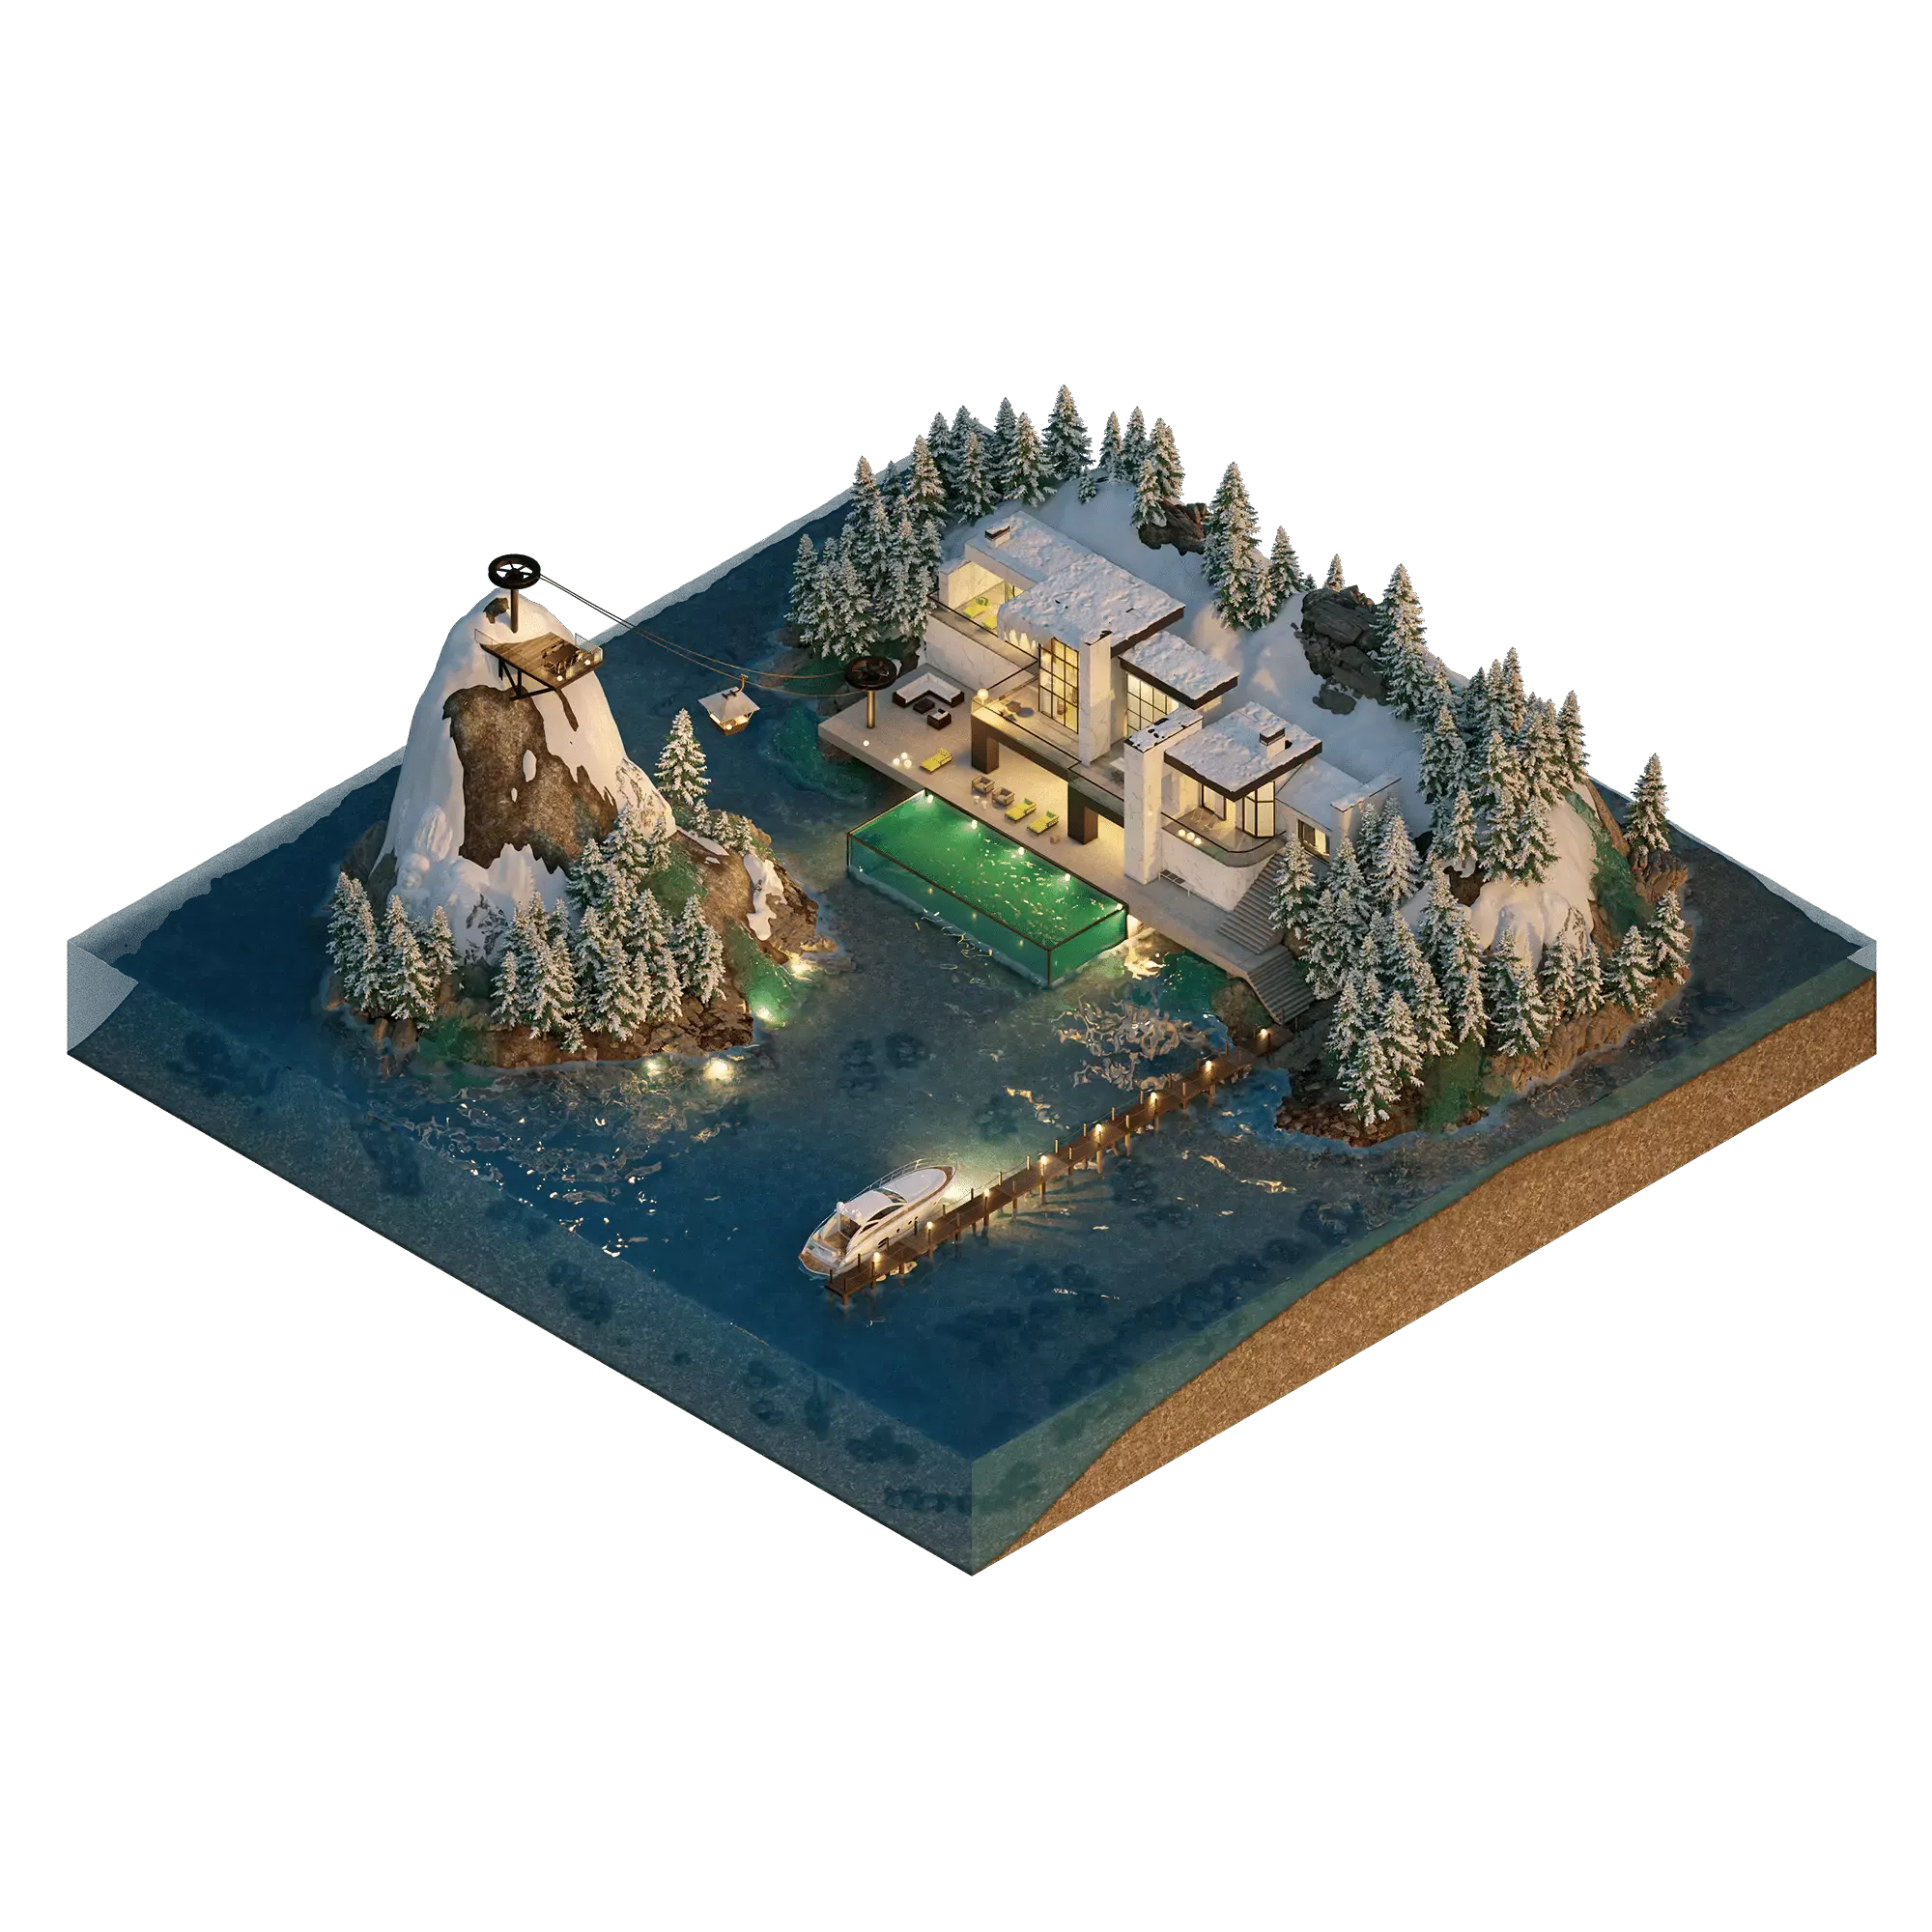
\includegraphics[width=\linewidth]{03-theory/everyrealm2022.png}
        \captionsetup{justification=justified}
        \caption{An example of a rare \textit{Fantasy Island} NFT \citep[from][]{everyrealm2022}}\label{fig: everyrealm2022}
    \end{minipage}
    \hfill
\end{wrapfigure}

This article also mentions that despite \$500,000,000 having been spent in 2021 on virtual land on platforms like The Sandbox, average land prices have decreased 91\% over the last 9 months since their peak in early December 2021, which occurred 1 month after Republic Realm's purchase of \$4.3 million \citep[]{kane2022}. How much of that `property' was bought by or let to retail investors hoping to become rich off of hard-earned savings, only to see 91\% depreciation in their virtual asset? 

What I hope to highlight in this section is that the `metaverse' is not what it is portrayed as. Its current co-option by (or perhaps origination in) the profit motive inherent to cryptocurrency-based metaverse platforms does not `liberate art', rather can lead to unenjoyable \citep{dejesus2022,delic2022}, exploitative , and hyper-commercialised practices \citep[]{ledesma2021,ongwesojr.2022,gach2022}. My criticism of these platforms is not to say that a diversity of media experiences, hosting a multiplicity of sociocultural narratives, from a variety of voices isn't welcome; rather the opposite. XR technologies, \gls{ar} specifically, due to its material and embodied relations, propose a real potential to provide a real type of embodied artistic liberation. But as Leddy and Puolakka note on Dewey Aesthetics \autoref{sec: theory-experience}, this liberation will never happen under the exploitative constraints of the capitalist modus operandi. Thus, for as long as both mega-corporations and cryptocurrency is are drivers for use of `space' in `the Metaverse', it will always mirror these conditions and be inherently flawed. Yet if we are to believe the marketing speak, it is in 'spaces' like these that technology companies foresee cultural production shifting to and flourishing in the next 10 years \citep[]{fatemi2022}. Although nascent in their implementation, and not widely known about, thankfully, mechanisms exist (see the Fediverse) to host open-source, federated communities away from the clutches and algorithmic abuse of `Big-Tech'. Until that happens in earnest, which is improbable due to the aversion by companies to harm profits, it leaves us wondering... \textit{What affect will the `Metaverse' have on the production, consumption, and dissemination of art of all types?}

\begin{figure}[ht]
    \centering
    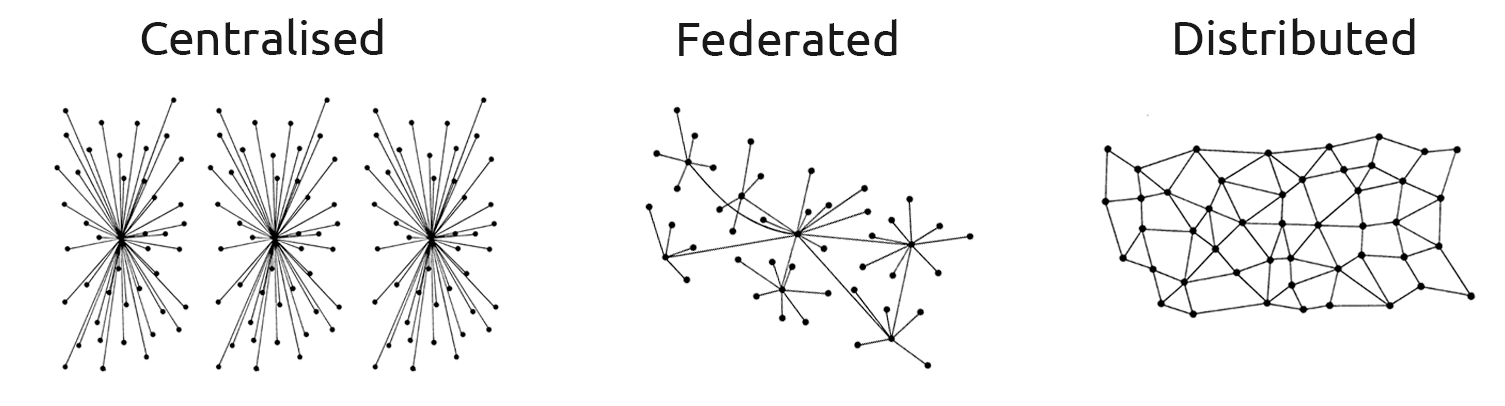
\includegraphics[width=.75\linewidth]{03-theory/baran1964.png}
    \captionsetup{justification=centering,margin=1.5cm}
    \caption{Different communication network types \citep[in][]{baran1964}}\label{fig: baran1964}
\end{figure}


In the next chapter I will outline the approach I have taken in my practice-based research to resist the current conception of `XR work \textit{as} the Metaverse'. This includes several forms of resistance, developing a DIY practice, creating and iterating on openly shared \gls{ar} experiences, and developing a set of design patterns to aid artists and musicians in employing \gls{ar} as a medium for creating similar work.